\documentclass[10pt,letterpaper]{article}
\usepackage[margin=0.7in]{geometry}
\usepackage{amsmath,graphicx,booktabs,float,caption}
\captionsetup{font=small,labelfont=bf}
\makeatletter\renewcommand\section{\@startsection{section}{1}{0pt}{-8pt}{3pt}{\normalfont\large\bfseries}}\makeatother
\setlength{\parskip}{3pt}
\title{\vspace{-1.2cm}A nearly uniform visible sphere: CoE profiles, shells and contrast limits}
\author{Addendum to the integrated model at $R=14.3$ Gpc}
\date{September 26, 2026}
\begin{document}
\maketitle\vspace{-0.9cm}

\section{Goal and scope}
The aim is a toy model of the Center of Expansion that explains the Hubble-flow anisotropy of Migkas et al.\ with ordinary gravity and ordinary matter. It has no dark matter, and baryons-only fits are preferred. It has no dark energy either, so the expansion is decelerating throughout. Fits that use an LCDM-equivalent matter density ($\Omega=0.3$) are shown only for comparison with the standard picture, and the CMB is set aside for now. The question here is whether the CoE model can match the observed dipole and quadrupole while the matter density across our visible sphere stays almost constant, as observed.

\section{Model and conventions}
The integrated model of the earlier addenda is kept: fixed-profile integration from $0.01\,t_0$, your geometry, and your sine term. It now has a compact CoE mass plus a uniform background of density $\Omega_b\rho_c$. The background is centred on the CoE, fixed in space and fills a sphere of radius $R_b=1.5(D+R)$, so every source lies inside it:
\begin{equation}\label{eq:eom}
\ddot{\mathbf x}=-\frac{G\,M_{\rm CoE}(<r)}{r^3}\,\mathbf x-\frac{4\pi}{3}G\Omega_b\rho_c\,\mathbf x \qquad (r<R_b).
\end{equation}
The CoE mass is unlabelled gravitating mass, so the model says nothing about whether it is baryonic or dark. The background is labelled ``LCDM-equivalent'' at $\Omega_b=0.3$, which is total matter and about 85\% dark, and ``baryons only'' at $\Omega_b=0.05$ (Planck $\Omega_bh^2=0.0224$, $h=0.7$). The uniformity limit applies to the total density across the visible sphere today,
\begin{equation}\label{eq:contrast}
\delta=\frac{\rho_{\rm tot}(D-R)-\rho_{\rm tot}(D+R)}{\rho_{\rm tot}(D)}\le 2\%\ \text{(main) or}\ 0.5\%\ \text{(strict)},
\end{equation}
and $\delta_{3.4}$ is the same ratio at $\pm3.4$ Gpc ($z\approx1$). The background pull in Eq.~(\ref{eq:eom}) is linear in $\mathbf x$, so the relative acceleration of any two particles is $-\tfrac{4\pi}{3}G\Omega_b\rho_c\,\Delta\mathbf x$, the same in every direction for every observer. With the CoE mass removed, the computed anisotropy of AF is $6\times10^{-9}$ for $\Omega_b$ from 0.1 to 1. All of the anisotropy therefore comes from the CoE mass through its $1/r^2$ tidal pattern, and the background only slows the flow uniformly. Migkas fit with a fixed cosmology, so their $A$ scales as $H_0^2$. Your sheet uses $A\propto{\rm AF}$, a velocity ratio, that is $A\approx1+\delta H/H$. We keep your convention, normalised to the sky mean as $A/A_{\rm all}$ is,
\begin{equation}\label{eq:A}
A(\theta)=\left[1-{\rm Amp}\sin(\theta+\varphi)\right]\frac{{\rm AF}^{p}}{\langle{\rm AF}^{p}\rangle_{\rm sky}},\qquad p=1\ \text{(your sheet)},\quad p=2\ \text{for}\ A\propto(H/H_0)^2\approx1+2\,\delta H/H,
\end{equation}
and report $p=2$ as a check. The age at $H_0=70$ is $t_0=(v_Et_0/r_E)/H_0$, and boundness is $(v_E/v_{\rm esc})^2\le1$ with the background potential included.

The other CoE profiles are, with $x=r/L$,
\begin{equation}\label{eq:profiles}
\rho\propto e^{-x},\quad (1+x)^{-n},\quad e^{-x^2/2},\quad \frac{1}{1+x^2},\quad e^{-(r-r_s)^2/2w^2},\quad G_\gamma(r/R_s)\ \ (\gamma=5/3,\,4/3),
\end{equation}
where $G_\gamma$ is the Sedov--Taylor self-similar density behind a strong spherical blast. It is integrated from the strong-shock jump conditions and checked to conserve the swept mass to $5\times10^{-4}$. For the ``point + ST shell'' case, a compact core $M_c$ of scale $L_c$ sits at the CoE, and a shell of constant density $\Omega_s\rho_c$ fills $R_{\rm in}<r<R_{\rm out}$ and replaces the background. Inside the shell
\begin{equation}\label{eq:ptshell}
g(r)=\frac{G\left[M_c+\tfrac{4\pi}{3}\rho_s\left(r^3-R_{\rm in}^3\right)\right]}{r^2}=\frac{4\pi}{3}G\rho_s\,r+\frac{G\left(M_c-M_{\rm hole}\right)}{r^2},\qquad M_{\rm hole}=\frac{4\pi}{3}\rho_sR_{\rm in}^3,
\end{equation}
so the linear term is isotropic, and the anisotropy comes only from the point mass minus the mass missing from the hole.

\section{Results}
The earlier unbound best fit already meets the limit once the background is added. Its contrast is 0.39\% and its $R^2$ barely moves (Table~\ref{tab:diag}). Without a background the same fit has an enormous contrast, because the visible sphere then contains nothing but the tail of the CoE profile. Refitting at $\delta\le2\%$ and $\le0.5\%$ gives $R^2=0.892$ with $\ell_0$ and 0.753 without, the same as the unconstrained unbound fits. The limit is active, with $\delta$ at the bound, but it costs less than 0.001 in $R^2$. It does rule out the extended bound solution of the previous note ($L/D\approx0.56$, $R^2=0.899$), whose contrast is 183\%. The constrained fits keep a compact CoE mass of 0.03--0.04 critical, about $1\times10^{24}\,M_\odot$, inside $D\approx40$ Gpc with $L\approx3$ Gpc. With $\Omega_b=0.3$ they are bound, 12.9--13.0 Gyr old, and turn around at 5.6--5.8 ages. They therefore satisfy the bound-and-age case (b) without change. With $\Omega_b=0.05$ (baryons only) the fit is unchanged in $R^2$, but Earth is unbound and the age is 13.6--13.8 Gyr. The boundness depends on how far the uniform background is assumed to extend. For the main fit $(v/v_{\rm esc})^2$ is 1.16, 0.48 and 0.12 for $R_b=1$, 1.5 and 3 times $D+R$. The dynamics and $R^2$ do not depend on $R_b$, because every particle stays inside it. Your literal $kR$ normalisation fails once the background is present ($R^2\le0.38$), because the uniform slowdown lowers the mean of your model A below 1.

All profiles that put their mass well inside $D-R$ fit equally well (Table~\ref{tab:prof}, Fig.~\ref{fig:prof}), because by Gauss's law the sources then see only the enclosed mass $M(<r)=M_{\rm CoE}$, whose local log-slope near $D$ is zero. What the fit does constrain is the depth of the central potential the particles climbed out of early on, $\Psi=G\int_0^\infty M(<r)\,dr/r^2$. This comes out at 0.15--0.32 in units of $GM_{\rm crit}/D$ for all the profiles that fit well, so compact profiles trade $M$ against their scale roughly as $M/L$ at fixed $\Psi$. The power law runs to its steepest index, and the Sedov--Taylor profiles put the front at $R_s\approx0.24\,D$, leaving the observer outside. Both are then indistinguishable from the exponential, and $\gamma$ makes no difference. A Gaussian shell at $r_s\approx0.25\,D$ is marginally best ($R^2=0.896$). The cored profile, whose mass keeps growing as $r$, is discussed in Section~\ref{sec:shell}. The point + ST shell fits as well as the rest. The fit drives the hole to nearly zero and the core to the smallest allowed size, so the result is again a compact mass inside a uniform medium. When the front is left free, it cuts through the visible sphere at a 100\% density step, which violates the limit. The squared convention, $p=2$, lowers $R^2$ by 0.004 and needs a smaller mass, as expected from the doubled response.

\begin{table}[H]\centering\scriptsize\setlength{\tabcolsep}{2.4pt}
\caption{Parameters of the $e^{-r/L}$ + background fits, vs the Migkas points with $\ell_0$ unless marked. $M/M_{\rm crit}$ is the CoE mass inside $D$ at $H_0=70$ today. Rows marked $\le2\%$ or $\le0.5\%$ apply Eq.~(\ref{eq:contrast}).}\label{tab:par}
\begin{tabular}{llccccccccccc}\toprule
Case & Matter & $D/R$ & $L/D$ & $D$ [Gpc] & $L$ [Gpc] & $M/M_{\rm crit}$ & $M$ [kg] & $M$ [$M_\odot$] & $\Omega_b$ & $\ell_0$ [$^\circ$] & Amp & $\varphi$\\\midrule
Previous best, no background & -- & 2.90 & 0.070 & 41.5 & 2.92 & 0.0273 & $2.21\times10^{54}$ & $1.11\times10^{24}$ & 0.00 & 13.2 & $-$0.051 & 0.75\\
Previous best + background & LCDM-equiv. & 2.90 & 0.070 & 41.5 & 2.92 & 0.0273 & $2.21\times10^{54}$ & $1.11\times10^{24}$ & 0.30 & 13.2 & $-$0.051 & 0.76\\
Unconstrained & LCDM-equiv. & 1.56 & 0.563 & 22.3 & 12.54 & 0.934 & $1.37\times10^{55}$ & $6.89\times10^{24}$ & 0.30 & 12.4 & $-$0.086 & 5.17\\
$\le2\%$, no $\ell_0$ & LCDM-equiv. & 2.67 & 0.086 & 38.2 & 3.28 & 0.0332 & $2.09\times10^{54}$ & $1.05\times10^{24}$ & 0.30 & 0.0 & $-$0.051 & 0.48\\
$\le2\%$ & LCDM-equiv. & 2.83 & 0.088 & 40.5 & 3.55 & 0.0389 & $2.94\times10^{54}$ & $1.48\times10^{24}$ & 0.30 & 13.1 & $-$0.049 & 0.71\\
$\le2\%$, vs $A_F$ & LCDM-equiv. & 2.68 & 0.084 & 38.3 & 3.22 & 0.0365 & $2.32\times10^{54}$ & $1.17\times10^{24}$ & 0.30 & 13.0 & $-$0.049 & 0.70\\
$\le2\%$, $\Omega_b$ free & free & 2.84 & 0.087 & 40.6 & 3.54 & 0.0386 & $2.93\times10^{54}$ & $1.47\times10^{24}$ & 0.29 & 13.1 & $-$0.049 & 0.72\\
$\le2\%$, $\Omega_b$ free, bound, age$\ge$12 & free & 2.83 & 0.103 & 40.4 & 4.16 & 0.0511 & $3.92\times10^{54}$ & $1.97\times10^{24}$ & 0.73 & 13.1 & $-$0.048 & 0.68\\
$\le0.5\%$, no $\ell_0$ & LCDM-equiv. & 2.74 & 0.071 & 39.2 & 2.78 & 0.0253 & $1.73\times10^{54}$ & $8.70\times10^{23}$ & 0.30 & 0.0 & $-$0.052 & 0.52\\
$\le0.5\%$ & LCDM-equiv. & 2.91 & 0.072 & 41.7 & 3.02 & 0.0297 & $2.43\times10^{54}$ & $1.22\times10^{24}$ & 0.30 & 13.2 & $-$0.051 & 0.75\\
$\le0.5\%$, vs $A_F$ & LCDM-equiv. & 2.75 & 0.070 & 39.3 & 2.74 & 0.028 & $1.92\times10^{54}$ & $9.66\times10^{23}$ & 0.30 & 13.1 & $-$0.051 & 0.74\\
$\le2\%$, no $\ell_0$ & baryons only & 2.75 & 0.068 & 39.4 & 2.66 & 0.0229 & $1.58\times10^{54}$ & $7.95\times10^{23}$ & 0.05 & 0.0 & $-$0.052 & 0.53\\
$\le2\%$ & baryons only & 3.18 & 0.010 & 45.4 & 0.45 & 0.00306 & $3.25\times10^{53}$ & $1.63\times10^{23}$ & 0.05 & 13.2 & $-$0.056 & 0.85\\
$\le0.5\%$, $\Omega_b$ free & free & 2.86 & 0.085 & 40.9 & 3.47 & 0.0388 & $3.16\times10^{54}$ & $1.59\times10^{24}$ & 0.98 & 13.1 & $-$0.050 & 0.73\\
$\le0.5\%$, $\Omega_b$ free, bound, age$\ge$12 & free & 2.92 & 0.071 & 41.7 & 2.97 & 0.0289 & $2.38\times10^{54}$ & $1.20\times10^{24}$ & 0.26 & 13.2 & $-$0.051 & 0.75\\
Literal $kR$, $\le2\%$, no $\ell_0$ & LCDM-equiv. & 3.06 & 0.010 & 43.7 & 0.44 & 0.00385 & $3.65\times10^{53}$ & $1.84\times10^{23}$ & 0.30 & 0.0 & $-$0.060 & 0.65\\
Literal $kR$, $\le2\%$ & LCDM-equiv. & 3.25 & 0.010 & 46.5 & 0.46 & 0.00429 & $4.89\times10^{53}$ & $2.46\times10^{23}$ & 0.30 & 13.4 & $-$0.061 & 0.86\\
\bottomrule\end{tabular}\end{table}

\begin{table}[H]\centering\scriptsize\setlength{\tabcolsep}{3pt}
\caption{Fit quality and physical checks for the rows of Table~\ref{tab:par}. Contrasts are in percent. Boundness uses $R_b=1.5(D+R)$. The age is at $H_0=70$, with a dagger below 12 Gyr. Turnaround is in units of the age. The last column confirms that no particle turns around before today.}\label{tab:diag}
\begin{tabular}{llcccccccc}\toprule
Case & Matter & $R^2_{\rm Migkas}$ & $R^2_{A_F}$ & $\delta$ [\%] & $\delta_{3.4}$ [\%] & $(v/v_{\rm esc})^2$ & Age [Gyr] & Turnaround & Outward today\\\midrule
Previous best, no background & -- & 0.892 & 0.976 & 13420 & 289 & 30.7 & 13.6 & $\infty$ & yes\\
Previous best + background & LCDM-equiv. & 0.891 & 0.975 & 0.387 & 0.00835 & 0.495 & 13.0 & 5.8 & yes\\
Unconstrained & LCDM-equiv. & 0.899 & 0.984 & 183 & 35.8 & 0.127 & 10.9$^\dagger$ & 2.5 & yes\\
$\le2\%$, no $\ell_0$ & LCDM-equiv. & 0.753 & 0.826 & 2 & 0.063 & 0.476 & 13.0 & 5.6 & yes\\
$\le2\%$ & LCDM-equiv. & 0.893 & 0.977 & 2 & 0.0794 & 0.483 & 12.9 & 5.7 & yes\\
$\le2\%$, vs $A_F$ & LCDM-equiv. & 0.892 & 0.977 & 2 & 0.0598 & 0.469 & 13.0 & 5.5 & yes\\
$\le2\%$, $\Omega_b$ free & free & 0.893 & 0.976 & 2 & 0.0788 & 0.5 & 13.0 & 6.0 & yes\\
$\le2\%$, $\Omega_b$ free, bound, age$\ge$12 & free & 0.893 & 0.976 & 2 & 0.117 & 0.187 & 12.2 & 2.9 & yes\\
$\le0.5\%$, no $\ell_0$ & LCDM-equiv. & 0.752 & 0.826 & 0.5 & 0.00902 & 0.485 & 13.0 & 5.7 & yes\\
$\le0.5\%$ & LCDM-equiv. & 0.892 & 0.976 & 0.5 & 0.0121 & 0.493 & 13.0 & 5.8 & yes\\
$\le0.5\%$, vs $A_F$ & LCDM-equiv. & 0.892 & 0.977 & 0.5 & 0.00853 & 0.478 & 13.0 & 5.6 & yes\\
$\le2\%$, no $\ell_0$ & baryons only & 0.752 & 0.826 & 2 & 0.0307 & 2.84 & 13.6 & $\infty$ & yes\\
$\le2\%$ & baryons only & 0.892 & 0.976 & 0 & 0 & 3.2 & 13.8 & $\infty$ & yes\\
$\le0.5\%$, $\Omega_b$ free & free & 0.893 & 0.977 & 0.5 & 0.0186 & 0.133 & 11.8$^\dagger$ & 2.5 & yes\\
$\le0.5\%$, $\Omega_b$ free, bound, age$\ge$12 & free & 0.892 & 0.976 & 0.5 & 0.0114 & 0.569 & 13.1 & 7.6 & yes\\
Literal $kR$, $\le2\%$, no $\ell_0$ & LCDM-equiv. & 0.193 & 0.223 & 0 & 0 & 0.495 & 13.2 & 5.8 & yes\\
Literal $kR$, $\le2\%$ & LCDM-equiv. & 0.377 & 0.422 & 0 & 0 & 0.501 & 13.2 & 5.9 & yes\\
\bottomrule\end{tabular}\end{table}

\begin{table}[H]\centering\scriptsize\setlength{\tabcolsep}{2.0pt}
\caption{CoE profile comparison at $\delta\le2\%$ with $\ell_0$, except the free-front row, which is unconstrained. $M/M_{\rm crit}$ is the CoE mass inside $D$ (for point + shell, the core $M_c$), and $\Omega$ is the background or shell density. $\Psi$ is the central potential depth of the CoE mass in units of $GM_{\rm crit}/D$. Shape lengths are in units of $D$; for point + shell (pt+shell) $R$ gives $R_{\rm in}$--$R_{\rm out}$. LCDM means the LCDM-equivalent $\Omega=0.3$ and baryons means $\Omega=0.05$. The last row uses $A\propto(H/H_0)^2$.}\label{tab:prof}
\begin{tabular}{lllccccccccccc}\toprule
Profile & Matter & Shape & $D/R$ & $M/M_{\rm crit}$ & $\Omega$ & $\ell_0$ & $R^2_{\rm Migkas}$ & $R^2_{A_F}$ & $\delta$ [\%] & $\delta_{3.4}$ [\%] & $\Psi$ & $(v/v_{\rm esc})^2$ & Age\\\midrule
e$^{-r/L}$ (main) & LCDM & $L$=0.088 & 2.83 & 0.0389 & 0.30 & 13.1 & 0.893 & 0.977 & 2 & 0.0794 & 0.22 & 0.483 & 12.9\\
e$^{-r/L}$ & baryons & $L$=0.010 & 3.18 & 0.00306 & 0.05 & 13.2 & 0.892 & 0.976 & 0 & 0 & 0.15 & 3.2 & 13.8\\
power law & LCDM & $L$=0.018, $n$=8.0 & 3.42 & 0.00152 & 0.30 & 13.3 & 0.893 & 0.977 & 0 & 0 & 0.21 & 0.549 & 13.3\\
Gaussian core & LCDM & $L$=0.179 & 2.67 & 0.0575 & 0.30 & 13.1 & 0.893 & 0.977 & 2 & 0.00209 & 0.25 & 0.464 & 12.8\\
cored & LCDM & $L$=0.010 & 9.93 & 0.0453 & 0.30 & 10.9 & 0.830 & 0.906 & 2 & 0.466 & 0.28 & 0.734 & 13.1\\
Gaussian shell & LCDM & $r_s$=0.25, $w$=0.097 & 2.37 & 0.0944 & 0.30 & 12.7 & 0.896 & 0.979 & 2 & 0 & 0.32 & 0.424 & 12.6\\
ST $\gamma=5/3$ & LCDM & $R_s$=0.241 & 2.73 & 0.0537 & 0.30 & 13.1 & 0.893 & 0.977 & 0 & 0 & 0.24 & 0.475 & 12.8\\
ST $\gamma=4/3$ & LCDM & $R_s$=0.241 & 2.73 & 0.0569 & 0.30 & 13.0 & 0.893 & 0.977 & 0 & 0 & 0.25 & 0.475 & 12.8\\
pt+shell, $\Omega_s$ free & free & $L_c$=0.005, $R$=0.02--3.94 & 3.29 & 0.00198 & 0.79 & 13.2 & 0.893 & 0.977 & 0 & 0 & 0.20 & 0.0439 & 12.4\\
pt+shell, $\Omega_s=0.3$ & LCDM & $L_c$=0.005, $R$=0.13--1.93 & 3.30 & 0.00185 & 0.30 & 13.2 & 0.893 & 0.977 & 0 & 0 & 0.18 & 0.552 & 13.3\\
pt+shell, $\Omega_s=0.05$ & baryons & $L_c$=0.005, $R$=0.08--3.97 & 3.28 & 0.00166 & 0.05 & 13.2 & 0.893 & 0.977 & 0 & 0 & 0.17 & 0.757 & 13.8\\
pt+shell, front free & free & $L_c$=0.005, $R$=0.93--1.59 & 3.51 & 0.00174 & 0.14 & 13.1 & 0.897 & 0.980 & $-$100 & $-$48.1 & 0.17 & 2.47 & 13.9\\
e$^{-r/L}$, $A\propto(H/H_0)^2$ & LCDM & $L$=0.010 & 3.22 & 0.00167 & 0.30 & 13.3 & 0.889 & 0.973 & 0 & 0 & 0.08 & 0.559 & 13.3\\
\bottomrule\end{tabular}\end{table}

\begin{figure}[H]\centering
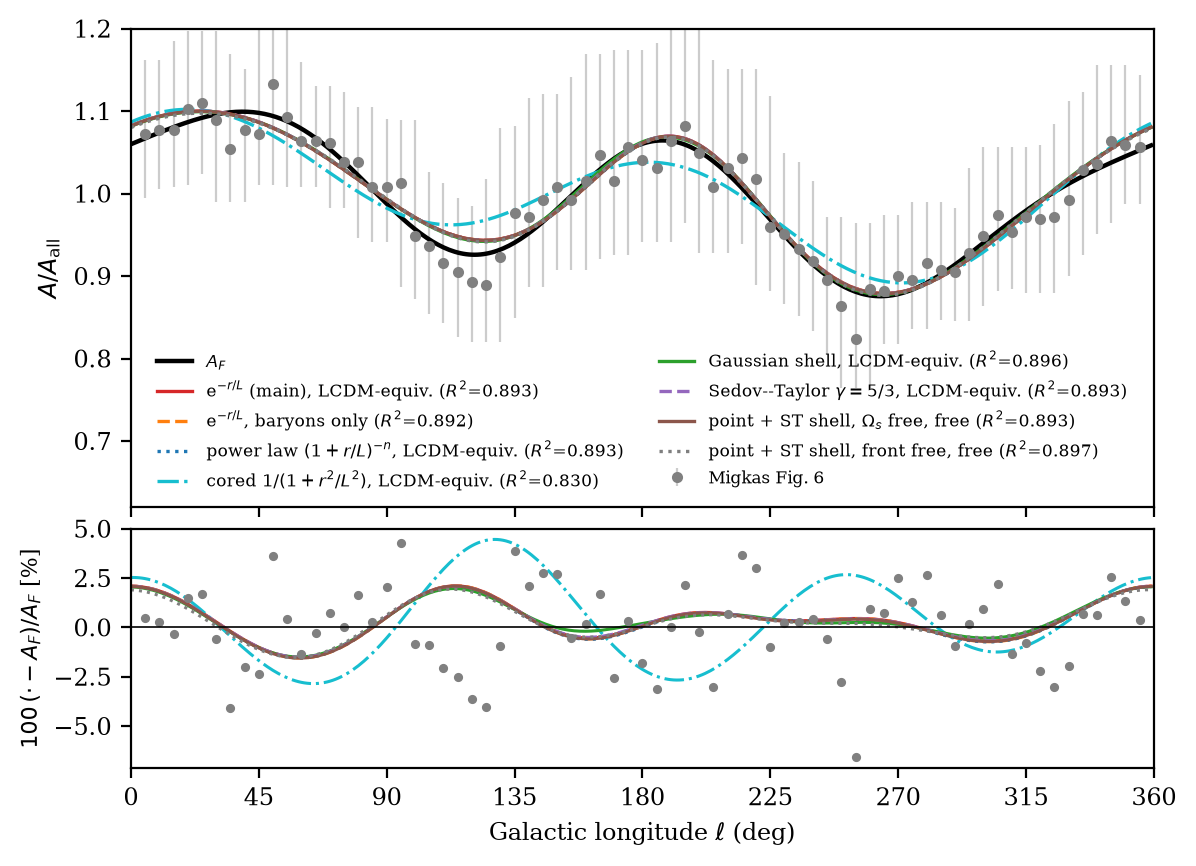
\includegraphics[width=0.72\textwidth]{uniform_bubble_profiles.png}
\caption{Best constrained fits for each CoE profile against the Migkas points and $A_F$. The lower panel shows percent differences from $A_F$. The compact profiles coincide.}\label{fig:prof}
\end{figure}

\begin{figure}[H]\centering
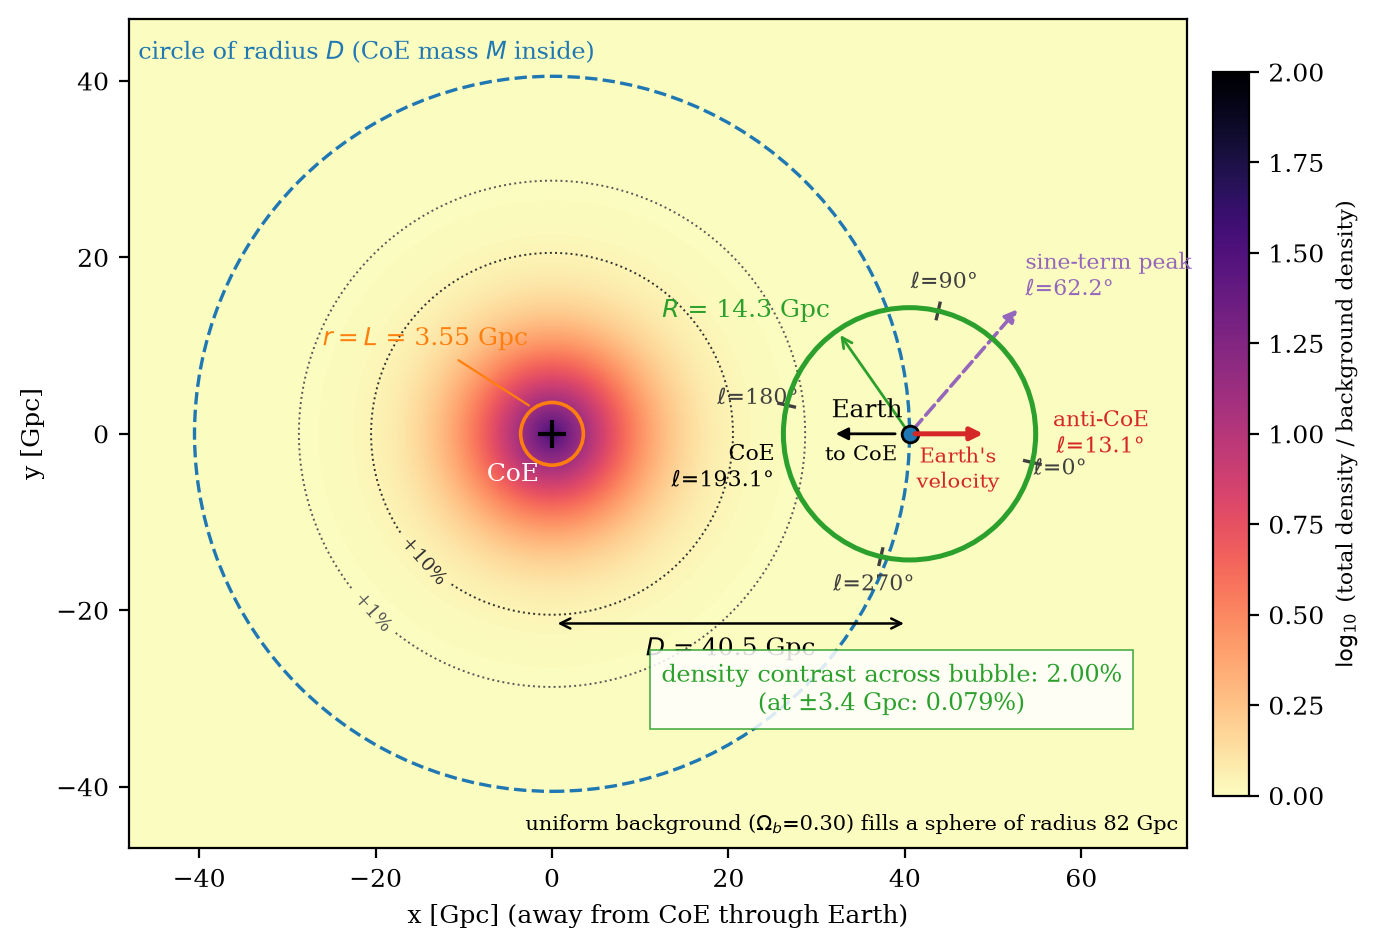
\includegraphics[width=0.66\textwidth]{uniform_bubble_drawing.png}
\caption{To scale, the $\delta\le2\%$ best fit with $\ell_0$ and $\Omega_b=0.3$. Shading is total density over background density on a log scale, and the dotted contours mark 1\% and 10\% above the background. The visible sphere (green) lies in the flat region.}\label{fig:draw}
\end{figure}

\section{Shell theorem, the cored profile and your thin shell}\label{sec:shell}
By Newton's shell theorem, symmetric matter inside radius $r$ acts as a point at the CoE, and symmetric matter outside $r$ exerts no net pull. Any symmetric distribution inside $D-R$ therefore acts on every source we see as a point mass, and only its total (plus the potential depth $\Psi$) can be measured. Symmetric matter beyond $D+R$ pulls on nothing we see. Only matter between $D-R$ and $D+R$ changes across the visible sphere, so a constant-density shell must be at least $2R$ thick, from $D-R$ to $D+R$, for the density there to be uniform. Inside such a shell Eq.~(\ref{eq:ptshell}) holds, and in the static field today the net central mass $M_c-M_{\rm hole}$ must be positive, or the tidal pattern reverses.

The cored profile $\rho\propto1/(1+(r/L)^2)$ is the equal-mass-shell picture: far from the core every shell of equal thickness holds the same mass, and $\rho\propto1/r^2$. It is a real fit. Its contrast across the visible sphere is
\begin{equation}\label{eq:cored}
\delta=D^2\left[\frac{1}{(D-R)^2}-\frac{1}{(D+R)^2}\right]=\frac{4R/D}{\left(1-R^2/D^2\right)^2}\approx\frac{4R}{D},
\end{equation}
which falls with distance (Table~\ref{tab:cored}). On its own, therefore, the cored profile meets the flat-density condition only far away. At $\delta\le2\%$ it needs $D=200R$ and gives $R^2=0.809$. With the $\Omega=0.3$ background it needs only $D=10.8R$ and gives $R^2=0.843$, which is 0.830 at the earlier cap $D/R\le10$. At $D\approx10R$ the cored profile alone has a contrast of about 40\%, so the background does most of the flattening there (Table~\ref{tab:alt}).

Your sketch puts a shell of constant density exactly around the visible sphere, $R_{\rm in}=D-R$ and $R_{\rm out}=D+R$, with an empty interior (Fig.~\ref{fig:thin}). We fitted it with the same integrator, with $D/R$, $\Omega_s$, $M_c$, $\ell_0$, Amp and $\varphi$ free, and also with the edges moved out by $0.1R$ (Table~\ref{tab:thin}). The sources start at 1\% of their present scale and move out through the fixed shell. The force uses the mass inside each particle's radius at each moment, so for most of the age the sources coast through the empty hole, where only the core pulls. They enter the shell only in roughly the last $R/D$ of the age. With a core, the shell fits well: $R^2=0.909$ at $\Omega_s=1.01$ and $D=94$ Gpc, the best of any model so far, bound and 13.8 Gyr old. At baryon density it gives $R^2=0.893$, the same as the best real-matter model, but Earth is unbound. The fitted net central mass is negative in every case, yet $\ell_0$ stays at $13^\circ$, because the core acted alone during the long coasting phase. With no core the pattern does turn, by about $90^\circ$ ($\ell_0=105$--$108^\circ$). This gives $R^2=0.83$ at $\Omega_s\approx1$ but only 0.33 at baryon density. The $0.1R$ margin changes nothing, and $p=2$ lowers $R^2$ by 0.003--0.009.

\begin{table}[H]\centering\small
\caption{Contrast of a pure $1/r^2$ (equal-mass-shell) profile across the visible sphere, Eq.~(\ref{eq:cored}).}\label{tab:cored}
\begin{tabular}{ccc}\toprule
$D/R$ & $4R/D$ [\%] & exact $\delta$ [\%]\\\midrule
3.3 & 121 & 147\\ 10 & 40 & 41\\ 50 & 8 & 8.0\\ 200 & 2 & 2.0\\\bottomrule
\end{tabular}\end{table}

\begin{table}[H]\centering\scriptsize\setlength{\tabcolsep}{1.6pt}
\caption{Cored and thin-shell fits compared with the best real-matter fit, all with $\ell_0$ free and $p=1$. Lengths in Gpc. $M$ is all gravitating mass inside $D$, and $r_s/D$ uses $r_s=2GM(<D)/c^2$. Thin shells run from $D-R$ to $D+R$.}\label{tab:alt}
\begin{tabular}{llccllcccccccc}\toprule
Model & Matter & $D/R$ & $D$ & Shape [Gpc] & $M$ [$M_\odot$] & $\Omega$ & $\ell_0$ & $R^2_{\rm Migkas}$ & $R^2_{A_F}$ & $\delta$ [\%] & $(v/v_{\rm esc})^2$ & Age & $r_s/D$\\\midrule
point + ST shell (best real matter) & baryons & 3.28 & 47 & $L_c$ 0.23; shell 3.7--187 & $3.04\times10^{24}$ & 0.05 & 13 & 0.893 & 0.977 & 0 & 0.76 & 13.8 & 6.2\\
cored $1/(1+(r/L)^2)$ + background & LCDM & 10.84 & 155 & $L$ 1.56 & $1.06\times10^{26}$ & 0.30 & 15 & 0.843 & 0.919 & 2 & 0.73 & 13.0 & 65\\
cored + background & baryons & 48.44 & 693 & $L$ 6.9 & $8.92\times10^{27}$ & 0.05 & 15 & 0.815 & 0.889 & 2 & 3.92 & 13.5 & 1{,}233\\
cored alone & none & 199.98 & 2860 & $L$ 28.7 & $6.21\times10^{29}$ & 0.00 & 15 & 0.809 & 0.882 & 2 & 12.82 & 13.6 & 20{,}795\\
thin shell + core & free & 6.55 & 94 & shell 79--108 & $1.86\times10^{26}$ & 1.01 & 13 & 0.909 & 0.987 & 0 & 0.90 & 13.8 & 190\\
thin shell + core & baryons & 3.47 & 50 & shell 35--64 & $2.34\times10^{24}$ & 0.05 & 13 & 0.893 & 0.977 & 0 & 10.56 & 13.9 & 4.5\\
thin shell only & free & 8.28 & 118 & shell 104--133 & $3.19\times10^{26}$ & 1.08 & 108 & 0.830 & 0.905 & 0 & 1.30 & 13.8 & 258\\
thin shell only & baryons & 3.77 & 54 & shell 40--68 & $2.71\times10^{24}$ & 0.05 & 105 & 0.332 & 0.368 & 0 & 13.30 & 13.9 & 4.8\\
\bottomrule\end{tabular}\end{table}

\begin{table}[H]\centering\scriptsize\setlength{\tabcolsep}{3pt}
\caption{Your thin shell, $R_{\rm in}=D-R$ and $R_{\rm out}=D+R$ (``margin'': $D\mp1.1R$). Masses are in units of $M_{\rm crit}(D)$, and $M_{\rm hole}=\Omega_s(R_{\rm in}/D)^3$. $p=2$ rows use $A\propto(H/H_0)^2$.}\label{tab:thin}
\begin{tabular}{llcccccccccc}\toprule
Case & Matter & $D/R$ & $\Omega_s$ & $M_c/M_{\rm crit}$ & $M_{\rm hole}/M_{\rm crit}$ & Net & $\ell_0$ [$^\circ$] & $R^2_{\rm Migkas}$ & $R^2_{A_F}$ & $(v/v_{\rm esc})^2$ & Age [Gyr]\\\midrule
shell only & free & 8.28 & 1.082 & 0.0000 & 0.7350 & $-$0.7350 & 108.0 & 0.830 & 0.905 & 1.30 & 13.8\\
shell only & baryons & 3.77 & 0.050 & 0.0000 & 0.0198 & $-$0.0198 & 105.0 & 0.332 & 0.368 & 13.30 & 13.9\\
shell $+$ core & free & 6.55 & 1.012 & 0.0027 & 0.6161 & $-$0.6135 & 12.8 & 0.909 & 0.987 & 0.90 & 13.8\\
shell $+$ core & baryons & 3.47 & 0.050 & 0.0017 & 0.0181 & $-$0.0163 & 13.2 & 0.893 & 0.977 & 10.56 & 13.9\\
shell only, margin & free & 8.62 & 1.034 & 0.0000 & 0.6866 & $-$0.6866 & 107.6 & 0.828 & 0.903 & 1.33 & 13.8\\
shell $+$ core, margin & free & 6.75 & 1.005 & 0.0027 & 0.5898 & $-$0.5871 & 12.8 & 0.909 & 0.987 & 0.84 & 13.8\\
shell $+$ core, margin & baryons & 3.43 & 0.050 & 0.0017 & 0.0157 & $-$0.0140 & 13.2 & 0.893 & 0.977 & 9.38 & 13.9\\
shell only, $p=2$ & free & 2.29 & 0.465 & 0.0000 & 0.0833 & $-$0.0833 & 288.0 & 0.821 & 0.901 & 0.88 & 13.4\\
shell $+$ core, $p=2$ & baryons & 3.69 & 0.050 & 0.0009 & 0.0194 & $-$0.0184 & 13.3 & 0.890 & 0.975 & 11.88 & 13.9\\
\bottomrule\end{tabular}\end{table}

\begin{figure}[H]\centering
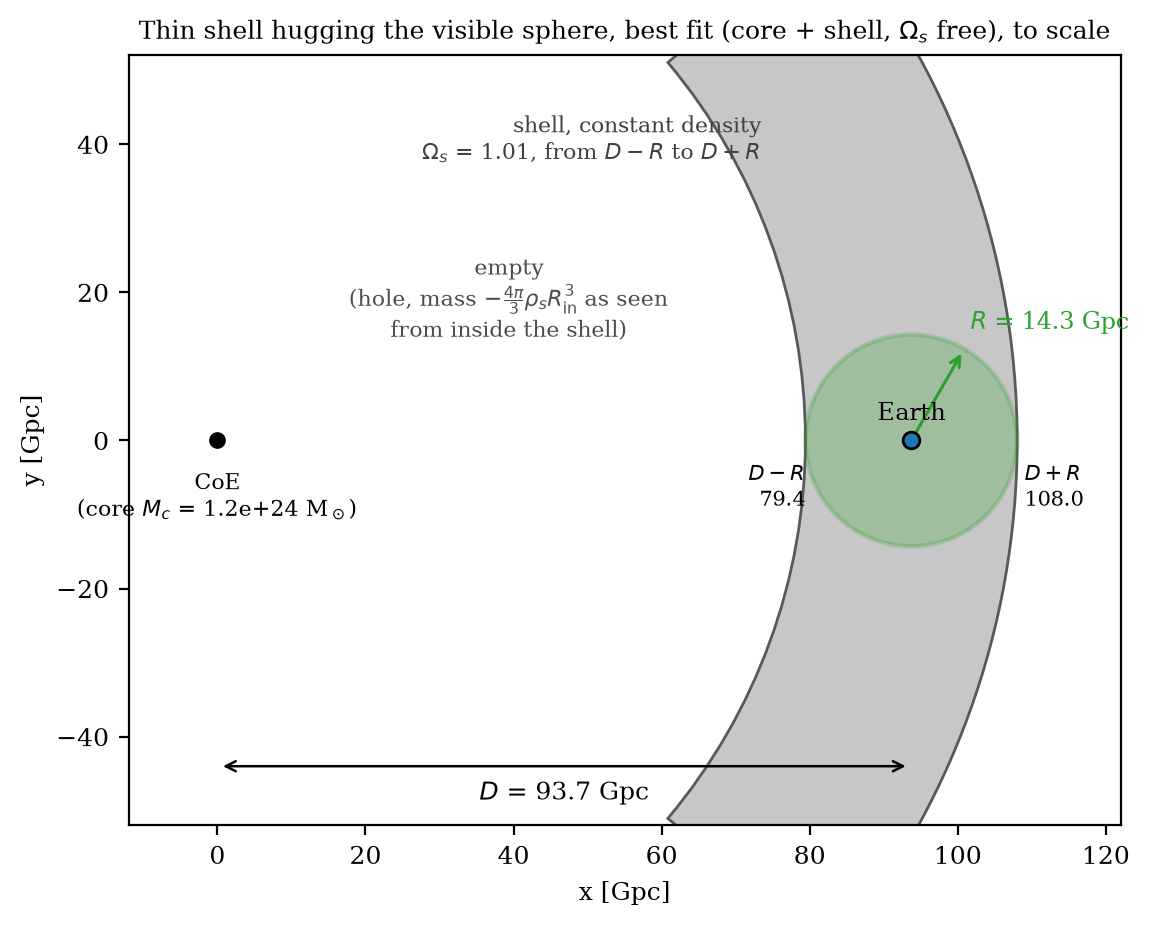
\includegraphics[width=0.49\textwidth]{thin_shell_drawing.png}\hfill
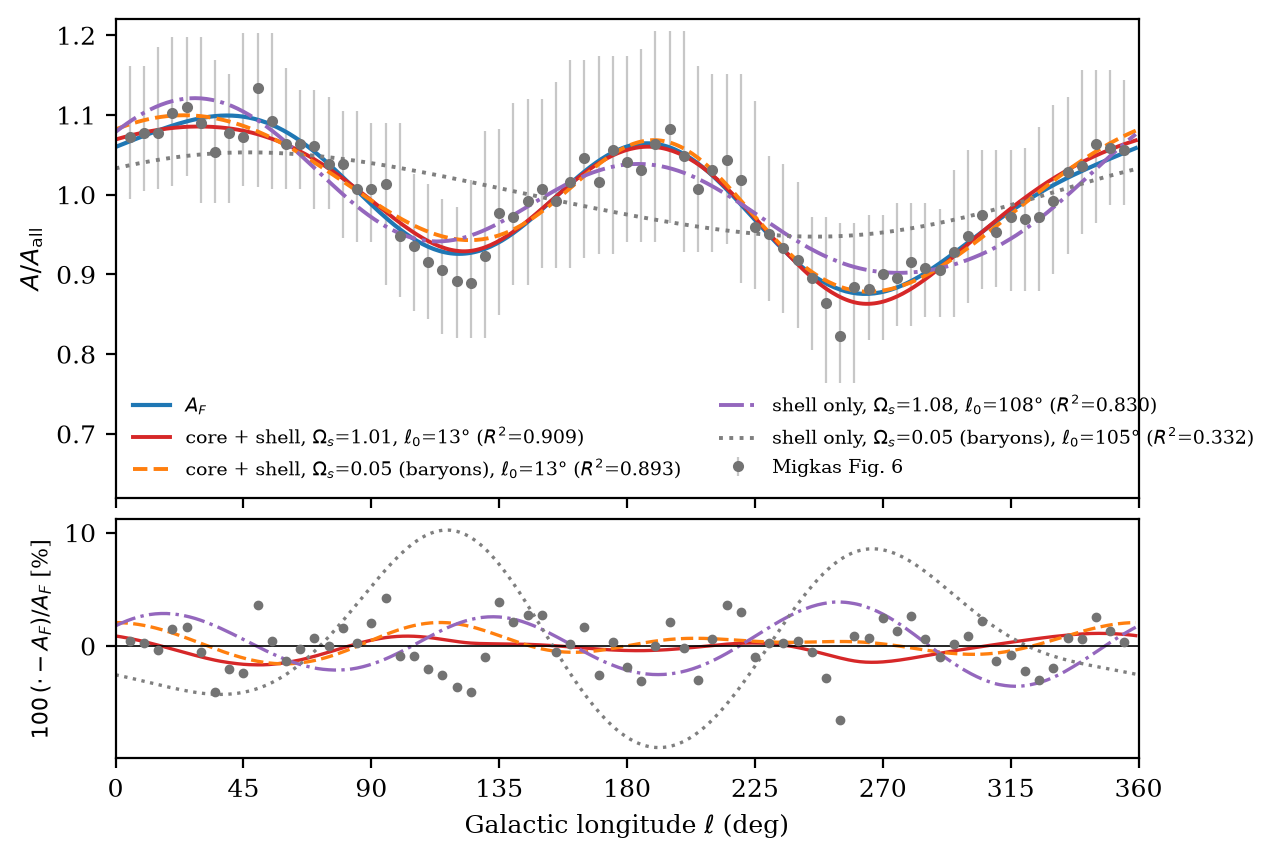
\includegraphics[width=0.49\textwidth]{thin_shell_Achart.png}
\caption{Left: your thin shell, to scale, at its best fit (core plus shell, $\Omega_s$ free). Right: thin-shell fits against the Migkas points and $A_F$.}\label{fig:thin}
\end{figure}
\end{document}
